%%%%%%%%%%%%%%
\section{Classificação Associativa}\label{sec:ca}
%%%%%%%%%%%%%%

A classificação associativa (CA) faz parte da família de algoritmos baseados em regras, os quais fazem uso das mesmas para representar o conhecimento extraído. No caso da CA, os algoritmos utilizam-se de um tipo especial de regra de associação (RA), conhecida como regra de associação classificativa (RAC), para realizar a indução do modelo. Uma RAC é uma regra do tipo $A \Rightarrow c$, na qual o antecedente ($A$) contém um conjunto de pares <atributo-valor> e o consequente (\textit{c}) uma das classes de um dado problema \cite{liu1998}. As mesmas são, em geral, extraídas via adaptação do algoritmo Apriori. A utilização destes algoritmos é vantajosa, uma vez que as regras contidas nos modelos são interpretáveis por especialistas que podem avaliá-las e tomar decisões com auxílio computacional. Segundo \citeonline{Padillo2020} estudos recentes têm demonstrado que a classificação associativa apresenta vantagens sobre as abordagens de classificação interpretáveis tradicionais. Devido a esta característica, dentre outras, diversas áreas vêm aplicando
classificadores associativos (CAs) nos últimos anos (vide \textit{review} de \citeonline{10.1016/j.eswa.2025.127454}). Além disso, tal como outras famílias de algoritmos, esforços vêm sendo realizados no sentido de popularizar ainda mais a CA por meio da implementação de pacotes, como visto, por exemplo, em \citeonline{Hahsler2019254}, \citeonline{Padillo2020}, e \citeonline{10.1145/3419604.3419762}, os quais contribuem ao disponibilizar algoritmos para uso geral. Segundo \citeonline{EasyChair:501}, o CBA \cite{liu1998} é o algoritmo mais utilizado da família e, portanto, o que se encontra disponível nos mais diversos pacotes.

A construção de um classificador associativo, via CBA, assim como na maioria dos demais algoritmos, ocorre em etapas, a saber: [a] extração de um conjunto de RACs; [b] ranqueamento das regras geradas; [c] poda das regras. No que se refere a etapa [a], em relação ao CBA, \citeonline{liu1998} apresentam uma adaptação do algoritmo Apriori para obtenção das RACs. No que se refere as demais etapas tem-se que:

%%%%%%%%%%%%%%%%%%%
\begin{description}
    %%%%%%%%%%%%%%%%%%%
    \item[Ranqueamento.] A partir das RACs extraídas, as mesmas são ordenadas de acordo com a relação $\succ$. Dado duas regras, $r_i$ e $r_j$, $r_i \succ r_j$, ou seja, $r_i$ tem maior precedência que $r_j$ se:
    
    \begin{enumerate}
        \item a confiança de $r_i$ for maior que a de $r_j$, ou
        \item se as confianças forem iguais, mas o suporte de $r_i$ for maior que o suporte de $r_j$, ou
        \item tanto a confiança como o suporte são iguais, mas $r_i$ foi gerada primeiro que $r_j$.
    \end{enumerate}
	
    %%%%%%%%%%%%%%%%%%%
    \item [Poda.] Para cada regra $r$, verifica-se as transações que ela cobre e se cobre corretamente pelo menos uma transação. Nesse caso, a regra é selecionada para ser incluída no modelo e todas as transações cobertas por ela são removidas.
\end{description}
%%%%%%%%%%%%%%%%%%%

A partir do modelo obtido, dada uma instância não vista, a classe associada à primeira regra que casa com a instância é a que será atribuído a ela. A Figura~\ref{fig:fluxo_cba} ilustra o fluxo descrito, incluindo a etapa de predição.

%%%%%%%%%%%%%%%%%%%%
\begin{figure}[H]
    \centering
    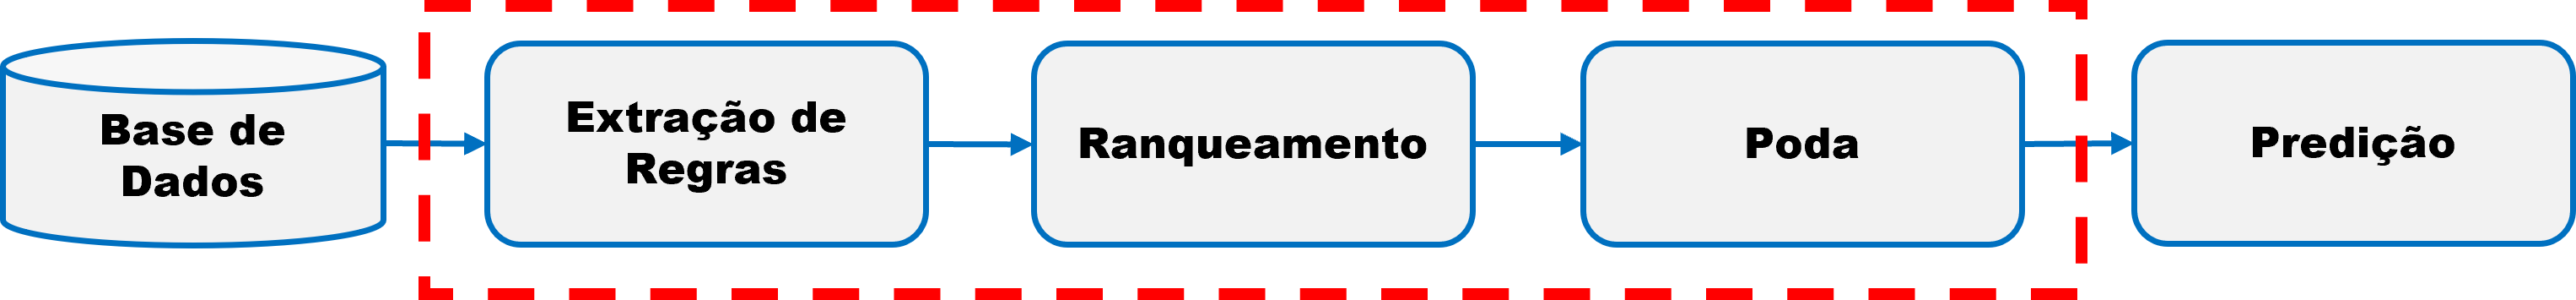
\includegraphics[width=\linewidth]{figuras/fluxo-geral.png}
    \caption{Etapas envolvidas na indução de um CA.}
    \label{fig:fluxo_cba}
\end{figure}
%%%%%%%%%%%%%%%%%%%%
